\documentclass[a4paper,11pt,twoside]{memoir}
\chapterstyle{veelo}

\usepackage{TUINFDA}

\usepackage{url}
\usepackage{hyperref}					% links in pdf
\usepackage{graphicx}            			% Figures
\usepackage{verbatim}            			% Code-Environment
\usepackage[lined,linesnumbered,algochapter]{algorithm2e} % Algorithm-Environment

\usepackage{pgf}
\usepackage{tikz}					% tikz graphics
\usetikzlibrary{arrows,automata}

\usepackage{ngerman}
\usepackage[ngerman]{babel}
\usepackage{bibgerm,cite}       % Deutsche Bezeichnungen, Automatisches Zusammenfassen von Literaturstellen
\usepackage[ngerman]{varioref}  % Querverweise
% to use the german charset include cp850 for MS-DOS, ansinew for Windows and latin1 for Linux.
% \usepackage[latin1]{inputenc}

\usepackage{rotating}

\thesistype{DIPLOMARBEITS-PROPOSAL}{MASTER'S THESIS PROPOSAL}
\thesistitle{TempMunger}
\thesissubtitle{A Visual Analytics Approach Supporting Transformations of Time-Oriented Data} % optional
\thesisdate{18.11.2012}

% all titles and designations have to be gender-related!
\thesisdegree{Diplom-Ingenieur}{Diplom-Ingenieur}
\thesiscurriculum{Informatik}{Computer Science} % your study
\thesiscurriculumlineone{Informatik -- Master -- 066 933}{Computer Science -- Master -- 066 933}
\thesiscurriculumlinetwo{Information \& Knowledge Management}
\thesisverfassung{Verfasser} % Verfasser
\thesisauthor{Robert Thurnher} % your name
\thesisauthoraddress{Neubaugasse 64-66, A-1070 Wien} % your address
\thesismatrikelno{0004297} % your registration number

\thesisbetreins{Univ.-Prof. Silvia Miksch}
\thesisbetrzwei{Dr. Theresia Gschwandtner}

% define page numbering styles
\makepagestyle{numberCorner}
\makeevenfoot{numberCorner}{\thepage}{}{}
\makeoddfoot{numberCorner}{}{}{\thepage}

% define custom macros for specific formats or names
\newcommand{\uml}[1]{\texttt{#1}}
\newcommand{\cd}{\textsf{Class Diagram}}

\begin{document}

\captionnamefont{\bfseries}

%%%%%%%%%%%%%%%%%%%%%%%%%%%%%%%%%%%%%%%%%
%%%   FRONTMATTER    %%%%%%%%%%%%%%%%%%%%
%%%%%%%%%%%%%%%%%%%%%%%%%%%%%%%%%%%%%%%%%
\frontmatter
\pagenumbering{roman}

%%%%%%%%%%%%%%%%%%%%%%%%%%%%%%%%%%%%%%%%%
%%%   TITLEPAGES    %%%%%%%%%%%%%%%%%%%%%
%%%%%%%%%%%%%%%%%%%%%%%%%%%%%%%%%%%%%%%%%

% the german title page is required as first page
% $Id: titlepage.tex 1752 2010-03-20 11:07:02Z tkren $
%
% TU Wien - Faculty of Informatics
% thesis titlepage
%
% This titlepage is using the geometry package, see
% <http://www.ctan.org/macros/latex/contrib/geometry/geometry.pdf>
%
% For questions and comments send an email to
% Thomas Krennwallner <tkren@kr.tuwien.ac.at>
% or to Petra Brosch <brosch@big.tuwien.ac.at>
%

\selectlanguage{english}

% setup page dimensions for titlepage
\newgeometry{left=2.4cm,right=2.4cm,bottom=2.5cm,top=2cm}

% force baselineskip and parindent
\newlength{\tmpbaselineskip}
\setlength{\tmpbaselineskip}{\baselineskip}
\setlength{\baselineskip}{13.6pt}
\newlength{\tmpparindent}
\setlength{\tmpparindent}{\parindent}
\setlength{\parindent}{17pt}

% first titlepage
\thispagestyle{tuinftitlepage}

%
% Kludge: for each titlepage set \pagenumbering to a different
% style. This is used to fix a problem with hyperref, because there
% are multiple "page 1" and hyperref hates that
%
\pagenumbering{Alph}

\begin{center}
{\ \vspace{3.4cm}}

\begin{minipage}[t][2.8cm][s]{\textwidth}%
\centering
\thesistitlefontHUGE\sffamily\bfseries \tuinfthesistitle\\
\bigskip
{\thesistitlefonthuge\sffamily\bfseries \tuinfthesissubtitle}
\end{minipage}

\vspace{1.3cm}

{\thesistitlefontLARGE\sffamily \tuinfthesistypeen}

\vspace{6mm}

{\thesistitlefontlarge\sffamily for the degree of}

\vspace{6mm}

{\thesistitlefontLARGE\sffamily\bfseries \tuinfthesisdegree}

\vspace{6mm}

{\thesistitlefontlarge\sffamily in}

\vspace{6mm}

{\thesistitlefontLarge\sffamily\bfseries \tuinfthesiscurriculumlineoneen\\\tuinfthesiscurriculumlinetwo}

\vspace{6.5mm}

{\thesistitlefontlarge\sffamily by}

\vspace{6mm}

{\thesistitlefontLarge\sffamily\bfseries \tuinfthesisauthor}

\vspace{1.5mm}

{\thesistitlefontlarge\sffamily Registration Number \tuinfthesismatrikelno}

\vspace{1.4cm}

\vspace{0pt}\raggedright\thesistitlefontnormalsize\sffamily
\begin{minipage}[t][1.6cm][t]{\textwidth}%
  %
  to the Faculty of Informatics

  at the Vienna University of Technology
\end{minipage}

\begin{minipage}[t][4cm][t]{\textwidth}%
  \vspace{0pt}\raggedright\thesistitlefontnormalsize\sffamily
  %
  \begin{tabbing}%
      \hspace{19mm} \= \hspace{66mm} \kill
      Advisor: \> \tuinfthesisbetreins\\
      Assistance: \> \tuinfthesisbetrzwei\\
                  \> \tuinfthesisbetrdrei
  \end{tabbing}
\end{minipage}

\begin{minipage}[t][1.5cm][t]{\textwidth}%
  \vspace{0pt}\sffamily\thesistitlefontnormalsize
  \begin{tabbing}%
    \hspace{45mm} \= \hspace{63mm} \= \hspace{51mm} \kill
    Wien, \tuinfthesisdate \> {\raggedright\rule{51mm}{0.5pt}} \\
    \> \begin{minipage}[t][0.5cm][t]{51mm}\centering (Signature of Advisor)\end{minipage}
    \end{tabbing}
\end{minipage}

\end{center}

% we want an empty page right after first titlepage
\pagestyle{empty}
\cleardoublepage

% we're done with the titlepages, proceed with default pagenumbering
\pagenumbering{roman}

% restore baselineskip
\setlength{\baselineskip}{\tmpbaselineskip}
\setlength{\parindent}{\tmpparindent}

% back to normal geometry
\restoregeometry


%%% Local Variables:
%%% TeX-PDF-mode: t
%%% TeX-debug-bad-boxes: t
%%% TeX-parse-self: t
%%% TeX-auto-save: t
%%% reftex-plug-into-AUCTeX: t
%%% End:


% an english translation may follow
%\include{titlepage_en} % optional

%%%%%%%%%%%%%%%%%%%%%%%%%%%%%%%%%%%%%%%%%
%%%   CONTENTS    %%%%%%%%%%%%%%%%%%%%%%%
%%%%%%%%%%%%%%%%%%%%%%%%%%%%%%%%%%%%%%%%%
% uncomment to set document language to german (results in "Inhaltsverzeichnis", "Kapitel", "Abbildung", etc. instead of "Contents", "Chapter", and "Figure"), otherwise the document's language is english
%\selectlanguage{ngerman}

\setcounter{tocdepth}{1}

\cleardoublepage
\pagestyle{numberCorner}
\tableofcontents*

%%%%%%%%%%%%%%%%%%%%%%%%%%%%%%%%%%%%%%%%%
%%%   MAINMATTER    %%%%%%%%%%%%%%%%%%%%%
%%%%%%%%%%%%%%%%%%%%%%%%%%%%%%%%%%%%%%%%%

\mainmatter
\pagenumbering{arabic}
\pagestyle{numberCorner}

%%%%%%%%%%%%%%%%%%%%%%%%%%%%%%%%%%%%%%%%%
\chapter{Abstract}
\label{ch:abstract}
%%%%%%%%%%%%%%%%%%%%%%%%%%%%%%%%%%%%%%%%%

\section{Problem Description}

Applied work within \textbf{Visual Analytics}, \textit{``the science of
analytical reasoning facilitated by interactive visual interfaces''}~\cite{Thomas2006}, can be seen to roughly consist of three main basic building blocks\footnote{\href{http://medriscoll.com/post/4740157098/the-three-sexy-skills-of-data-geeks}{Cf. http://www.dataspora.com/2009/05/sexy-data-geeks/}}:
\begin{enumerate}
  \item Statistics \& machine learning
  \item \textbf{Data wrangling} a.k.a. \textbf{munging}
  \item Visualization \& analysis itself
\end{enumerate}

While the first and last mentioned fields are constantly evolving related tools and techniques, the second one is comparatively still a bit lacking. This is when it comes down to actually wrangle usually messy real-world data into a format prepping it useful for analysis.

Currently, it mostly means fiddling around with the data manually, applying hand-crafted transformation scripts. This is a tedious task and discourages analyzing data altogether, especially if the ones intending to work on are not technically expertized (for instance, journalists).

However, combining contemporary knowledge and technology from the domains of \textbf{Human-Computer Interaction} (HCI) \& \textbf{User Experience} (UX) as well as \textbf{Information Retrieval} (IR)~\cite{Manning2008}, \textbf{Data Mining} / \textbf{Machine Learning} (ML)~\cite{Witten2011}, and \textbf{Visual Analytics} (VA) could yield substantial improvements here. Namely, making data wrangling accessible to a wider audience, mainly by providing a combination of analytical and visual methods to support the task of data munging. In this thesis we are going to scientifically investigate the field of data wrangling, plus, design, and prototypically implement a Visual Analytics approach to support this task.

That is, iteratively creating a software prototype which enables users to munge data suitable for analysis in a way which is as agile, intuitive, interactive, and overall visual as possible, respectively reasonable~\cite{Norman2002}.

Additionally, the to-be-developed prototype shall, in particular, make it convenient to work on \textbf{time-oriented datasets}. Time and time-oriented data have distinct characteristics that make it worthwhile to treat it as a separate data type~\cite{Aigner2011}.

\subsection{Research Questions}

So, the main research question is:

\textbf{\textit{In what way can we support data munging with Visual Analytics techniques?}}
\\\\
Plus, sub hypotheses being connected to design/implementation details. E.g.:

\begin{itemize}
  \item \textit{Which data transformations are best supported by analytical methods and for which transformations is visual support beneficial?}
  \item \textit{How do concrete data munging workflow processes look like and and how can these processes be supported by VA methods?}
  \item \textit{What data munging tasks need to be tackled in particular when dealing with time-oriented data and how can we support them with VA methods?}
\end{itemize}

The emphasis of this thesis lays on evaluating the feasibility of corresponding concepts via iterative design, implementation, and evaluation of a software prototype.


\section{Expected Results}

Results to be achieved will be:

\begin{itemize}
  \item Design and implementation of a research prototype
  \item Related evaluation and findings
  \item Detailed documentation of these
\end{itemize}

At the end of the project, it should be known whether developing such a tool in the described context is feasible and if so, how in detail. As mentioned above, the \textbf{prototype} shall combine concepts from HCI \& UX with ones from IR, ML, \& VA. Special focus will be put on crafting the \textbf{UI} and an underlying \textbf{analytical inference engine} interactively providing the user with respective data transform suggestions visually. Furthermore, \textbf{direct manipulation} of data should be easy. Plus, transformations shall, generally, be easily repeatable/-usable. A central challenge is making this all work in the context of time-oriented data (see above).

Answers to the stated research questions should be given, by designing, implementing, and evaluating a research prototype which provides VA techniques to improve and support data munging tasks.


\section{Method}
In order to answer our research questions we go for these concrete scientific methods:

\begin{enumerate}
  \item \textbf{Requirements analysis}
  \item \textbf{Design of UI \& interactions}
  \item \textbf{Iterative prototypical implementation}
  \item \textbf{Qualitative evaluation of results}
\end{enumerate}

Thus, the whole development process of the prototype should be conducted iteratively in an \textbf{agile} manner until satisfying results are achieved.

In the end, it should all be thoroughly documented emphasizing findings of the evaluation and lessons learned. The thesis will cover all aspects and findings of the development and evaluation of the prototype from UI/interaction mockups to architectural diagrams.

\subsection{Implementation}
Technically, the prototype will be a \textbf{web-based} application which can be run locally as well.
\\

The backend will at its core be powered by \textbf{Elasticsearch}\footnote{\href{https://www.elastic.co/products/elasticsearch}{https://www.elastic.co/products/elasticsearch}}, a high-performance search and data storage engine with strong, real-time analytics capabilities. Inference and probably transform operations of the backend will be based on \textbf{Apache Spark}\footnote{\href{https://spark.apache.org/}{https://spark.apache.org/}}, a fast engine for large-scale data processing with convenient access to ML algorithms via its \textbf{MLlib}. Spark integrates nicely with Elasticsearch via native support provided by ES for Hadoop project. The backend will expose a RESTful API built with \textbf{Kotlin}\footnote{\href{http://kotlinlang.org/}{http://kotlinlang.org/}}, Gradle build system, and \textbf{Spring Boot} framework.

The frontend will be a modern universal web browser app utilizing HTML5 with interactive charts via \textbf{SVG}, transpiled CSS, and \textbf{ES6}(+)-flavored JS. Probable technologies and patterns:\\
Node.js, Gulp tasks, Webpack, Babel, \textbf{Redux/React} architecture, material design UI kit, \textbf{D3.js}...


\section{State of the Art}

Basics of the field are laid out in \cite{dasu2003exploratory}, mainly related to classic extract, transform, and load (\textbf{ETL}) processes as known from \textbf{data warehousing}. General theoretical foundation of transforming large amounts of data interactively can be found in \cite{Dasu:2002:MDS:564691.564719}, and more recently \cite{hellerstein_quantitative}.

A system pioneering this area is \textit{Potter's Wheel}~\cite{Raman2001a} from 2001. Yet, among other things, it doesn't support ``fill'' transform operations (i.e., automatically filling certain fields with certain data, batch-wise) and, naturally, its usability is not up to modern standards. So, this tool resembles quite much the look \& feel of a Java Swing GUI application from the late 1990s, early 2000s (which, as a matter of fact, it happens to be).

The two systems which can claim to represent the current state of the art here are:

\begin{enumerate}
  \item \textbf{\textit{DataWrangler}}~\cite{Kandel2011a} (Stanford Visualization Group research project\footnote{\href{http://vis.stanford.edu/wrangler/}{http://vis.stanford.edu/wrangler/}})
  \item \textbf{\textit{OpenRefine}}~\cite{web:OpenRefine} (open-sourced product f.k.a. \textit{Google Refine}, f.k.a. \textit{Freebase Gridworks})
\end{enumerate}

\textit{DataWrangler} is a web-browser-based app very much oriented towards a visually interactive approach to some extent similar to our proposed one. It contains an inference engine suggesting transforms and data cleaning sessions can be exported and reused as scripts. One thing which is not really supported by Wrangler is direct manipulation of data. In addition to that, the UI is sort of limited which can also be ascribed to the web-based nature of the tool. Things like not truly responsively and richly interactive UX, especially when amounts of to be wrangled data grow.

\textit{OpenRefine} is a browser-based app as well (but running locally on the user's machine, mainly due to data privacy reasons). It allows for direct manipulation of data, yet, doesn't support as purely by interaction driven transform operations as Wrangler (receiving very appropriate transformation suggestions solely by pointing the cursor to data in a certain way). A nice feature is its visual statistical analytics of data distributions via histograms etc. But it generally lacks some data transformation operations which Wrangler has (especially reshaping-related, like un/folding -- extracting/merging specific parts of data within a column into/from additional ones).
\\

Where we're intending to excel with \textbf{\textit{TempMunger}} here is by bringing concepts from both Wrangler and Refine together with our own ideas and improved UX with respect to VA techniques, plus, focusing on specific munging tasks and support needed when dealing with time-oriented data.

Intended features of our prototype include:

\begin{itemize}
  \item Drag \& drop column merging
  \item Visualizing data structures via meaningful charts
  \item Directly manipulative interaction with these charts to transform underlying data
\end{itemize}

We think that further reasonable functionality will emerge from the iterative \textit{design -- implementation -- evaluation} process.


\section{Topic Match}

The thesis topic is a good match for the master's studies in computer science of \textit{``Information \& Knowledge Management''} because this program can somehow be seen as a blend of the master's of \textit{``Computational Intelligence''} with the one of \textit{``Software Engineering''}.

The topic relates closely to Software Engineering as it's in its essence an advanced, extensive software development project focusing on UI features, the efficient communication of information, and efficient support of user tasks, intending to answer given research questions in the field of VA.
Moreover, it relates to Computational Intelligence due to its close relationship with applied, contemporary Data Mining / ML, IR, analytical, and visual methods.


%%%%%%%%%%%%%%%%%%%%%%%%%%%%%%%%%%%%%%%%%
% \chapter{Appendix}
% \label{ch:appendix}
%%%%%%%%%%%%%%%%%%%%%%%%%%%%%%%%%%%%%%%%%

% \section{Rough Work Plan}

The thesis project will, organizationally, be split up into somewhat sprint-like chunks (agile methodology).
Each such \textbf{iteration} will have a duration of \textbf{approx. 4 weeks} and a concrete topic to work on.
At the end of an iteration the results will be reviewed and based on the outcome here the topic for the next one determined. Depending on requirements/circumstances it can also be decided that a respective iteration takes some more or some less time (that is, \textbf{+/- 2 weeks}).
Additionally, an iteration will have some more detailed topic/goal description if respectively applicable.

The whole project shall be finished \textbf{at latest by the end of 2013}.

Though, \textbf{optimistic intent} is to be done by \textbf{summer 2013} already.

The topic of the first iteration is: \textit{``Create Master's Thesis Proposal''}.

It's fluently followed by the 2nd iteration: \textit{``Literature Research \& State of the Art Report''}.

After that, initial actual UI design and implementation of basics of the app should begin.

All in all, there will be around \textbf{8 to 10 iterations} --
consisting of research, analysis, design, implementation, evaluation, and documentation (potentially overlapping and conjoined/intertwined).

Figure~\ref{fig:gantt} shows some Gantt chart diagram visualizing a \textbf{draft project plan}. Provisionally \textit{``Refine...''}-titled iterations can be seen to be generally optional or possibly included within previous iterations, respectively.

\begin{sidewaysfigure}[tb]
  \centering
  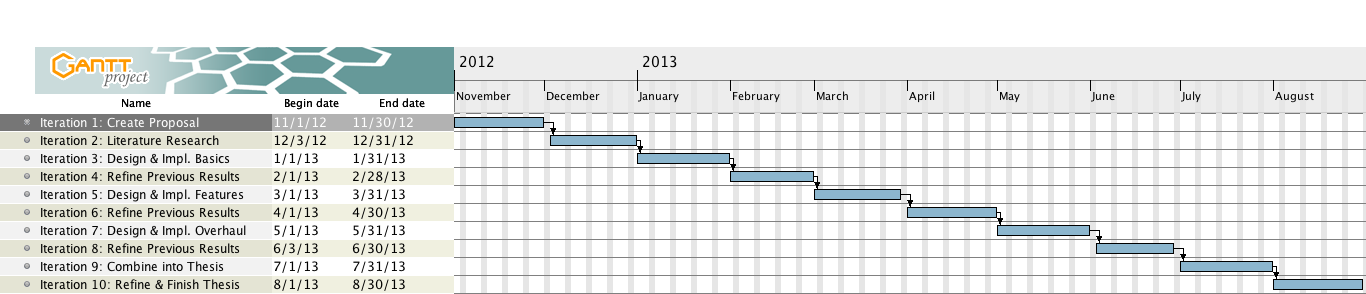
\includegraphics[width=1.0\textwidth]{figures/gantt-draft-project-plan}
  \caption{Draft Gantt chart diagram project plan}
  \label{fig:gantt}
\end{sidewaysfigure}


\section{Preliminary Thesis Structure}

\textbf{N.B.: }this is all subject to change while actually progressing with the thesis project.

\begin{itemize}
  \item Introduction
  	\begin{itemize}
  		\item motivation
  		\item problem statement (which problem should be solved?)
  		\item aim of the work
  		\item methodological approach
  		\item structure of the work
  	\end{itemize}
  \item State of the art / analysis of existing approaches
  	\begin{itemize}
  		\item literature studies
  		\item analysis
  		\item comparison and summary of existing approaches
  	\end{itemize}
  \item Methodology
  	\begin{itemize}
  		\item used concepts
  		\item methods and/or models
  		\item languages
  		\item design methods
  		\item data models
  		\item analysis methods
  		\item formalisms
  	\end{itemize}
  \item Design and implementation of the suggested solution
  \item Critical reflection
  	\begin{itemize}
  		\item comparison with related work
  		\item discussion of open issues
  	\end{itemize}
  \item Summary and future work
  \item ...
\end{itemize}


%%%%%%%%%%%%%%%%%%%%%%%%%%%%%%%%%%%%%%%%%
%%% BACKMATTER %%%%%%%%%%%%%%%%%%%%%%%%%%
%%%%%%%%%%%%%%%%%%%%%%%%%%%%%%%%%%%%%%%%%

\appendix

\bibliographystyle{plain}
\bibliography{references}

\end{document}
